\section{Review of state of the research field}
\label{sec:review}

%\begin{wrapfigure}[14]{R}[0pt]{0.6\textwidth}
% R - floating; r - h! [narrow lines] <- reduce whitespace below [17]
%  \centering
%  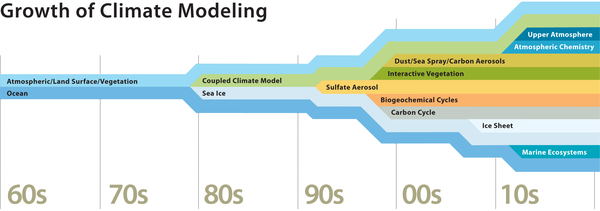
\includegraphics[width=0.58\textwidth]{evolution_of_climate_models}
%  \caption{A growth and evolution timeline of climate models. The complexity of global climate models has increased enormously over the last four decades. The most powerful models, such as the \gls{cesm}, now have the capability of simulating a broad range of atmospheric processes, such as the impact of marine ecosystems on the atmosphere. \copyright \gls{ncar}.}
%  \label{fig:growth_esm}
%\end{wrapfigure}

\textbf{\glspl{esm} have been rapidly evolving} over the past decades (Fig.~\ref{fig:growth_esm}) due to growing computational resources. Over time the scope of the models has substantially broadened and the physical realism of the models has steadily increased, among others due to improvements in resolution, grid types, parameterizations, and couplers \parencite{AMS:Randall2018}. But this development comes at the cost of a complexity rivaling the real world and immense resources for computing. To predict the response of the Earth’s ecosystem in a changing climate and its feedback on the very same climate, it is important to update model parameterizations to reflect the state-of-the-art scientific understanding of the underlying processes. From solving the Navier-Stokes equations of wind and waves several decades ago, \glspl{esm} came to represent even biotical process of soil microbial and fungi. But the more we learn the more do we know what is left unknown. At present \textbf{missing links and knowledge gaps exist especially when it comes to the details of the complex interaction between terrestrial ecosystems and the atmosphere} \textbf{\color{red}TODO: Add reference}. First analyses of the \gls{cmip} phase~6 indicate a growing divergence between models \parencite{ESD:Tebaldi2021}, in particular in the land and atmospheric components. Although this will not revoke our fundamental understanding of climate change, it still affects the reliability of model projections.\\

\begin{figure}[!ht]
  \centering
  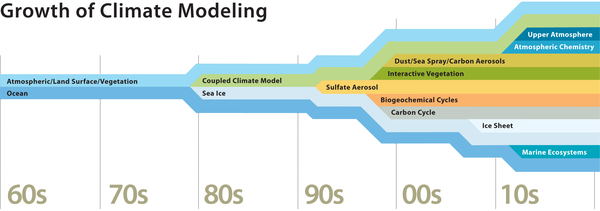
\includegraphics[width=0.68\textwidth]{evolution_of_climate_models}
  \caption{A growth and evolution timeline of climate models. The complexity of global climate models has increased enormously over the last four decades. The most powerful models, such as the \gls{cesm}, now have the capability of simulating a broad range of atmospheric processes, such as the impact of marine ecosystems on the atmosphere. \copyright \gls{ncar}.}
  \label{fig:growth_esm}
  \vspace*{-10pt}
\end{figure}


\textbf{The chemical composition of the atmosphere is complex} and the concentration of many important trace gases is highly variable in time and space and substantially influenced by natural and anthropogenic emissions. While increases in the concentrations of well-mixed greenhouse gases such as carbon dioxide (\ch{CO_2}) and methane (\ch{CH_4}) due to human activity are understood as the prime cause of climate warming, anthropogenic activity has also substantially affected the atmospheric composition and concentration of many other chemical species, many of which have important radiative properties.

One of these chemical species is \textbf{ozone, an important trace gas in the lower and middle atmosphere}, and central to this proposal. In accordance with its effects and realm of occurence, we can distinguish the good (stratosphere), \emph{the bad} (troposphere), and \emph{the ugly} (ambient air) ozone throughout the atmosphere. Here we focus on the connection and feedback between the bad and ugly sides of ozone. After carbon monoxide (\ch{CO_2}) and oxides of nitrogen (\ch{CH_4}) ozone (\ch{O_3}) is ranked third amongst the most potent climate forcers \parencite{IPCC2013c8}.
It contributes to warming in the troposphere where it \textbf{is produced as a secondary air pollutant} in chemical cycles involving precursors such as \ch{CO} and \ch{NO_x} as well as hydrocarbons -- often refered to as \gls{voc} and \gls{bvoc} in this context. Ozone is highly toxic and \textbf{harmful to human health and many ecosystems}. Model projections show diverse futures for surface ozone burdens under the \gls{rcp} scenarios, in sign and magnitude strongly dependent on changes in precursor emissions and climate \textbf{\color{red}TODO: Add references: general Reference} \parencites{JGR:Rieder2015}{AE:Rieder2018}{Nat:Skeie2020}. Projections of effects of future ozone air quality on human health and crop damage dependent on the level of ambition in both climate protection and precursor reduction \parencite{PTRS:Schneidemesser2020}.

Despite a successful reduction of precursors in recent years leading to a stagnation of the upward trend in tropospheric ozone concentrations, there are \textbf{indications that climate feedback on the ozone uptake by the land biosphere can hamper reaching air quality goals} \parencite{NCC:Lin2020}. Under drought conditions, plants will limit their transpiration by closing their stomata, which regulate all of their gas exchange. At the same time, such stressed vegetation is emitting \glspl{bvoc}, an important precursor, and thus increasing ozone concentrations \ch{[O_3]} in ground-level air. A high uptake of ozone will also lead to a reduction of stomatal opening and thus rival or even mitigate drought effects \parencite{BGS:Peron2021}. As ozone uptake through plants’ stomata is considered one of the most effective removal pathways, \textbf{stomatal closure under combined thermal and ozone stress will lead to a twofold penalty of climate change on vegetation and air quality}. At present however, large uncertainties in non-stomatal removal remain \parencite{RG:Clifton2020}.

%\begin{wrapfigure}[26]{R}[0pt]{0.5\textwidth}
% R - floating; r - h! [narrow lines] <- reduce whitespace below [17]
\begin{figure}[b]
  \centering
  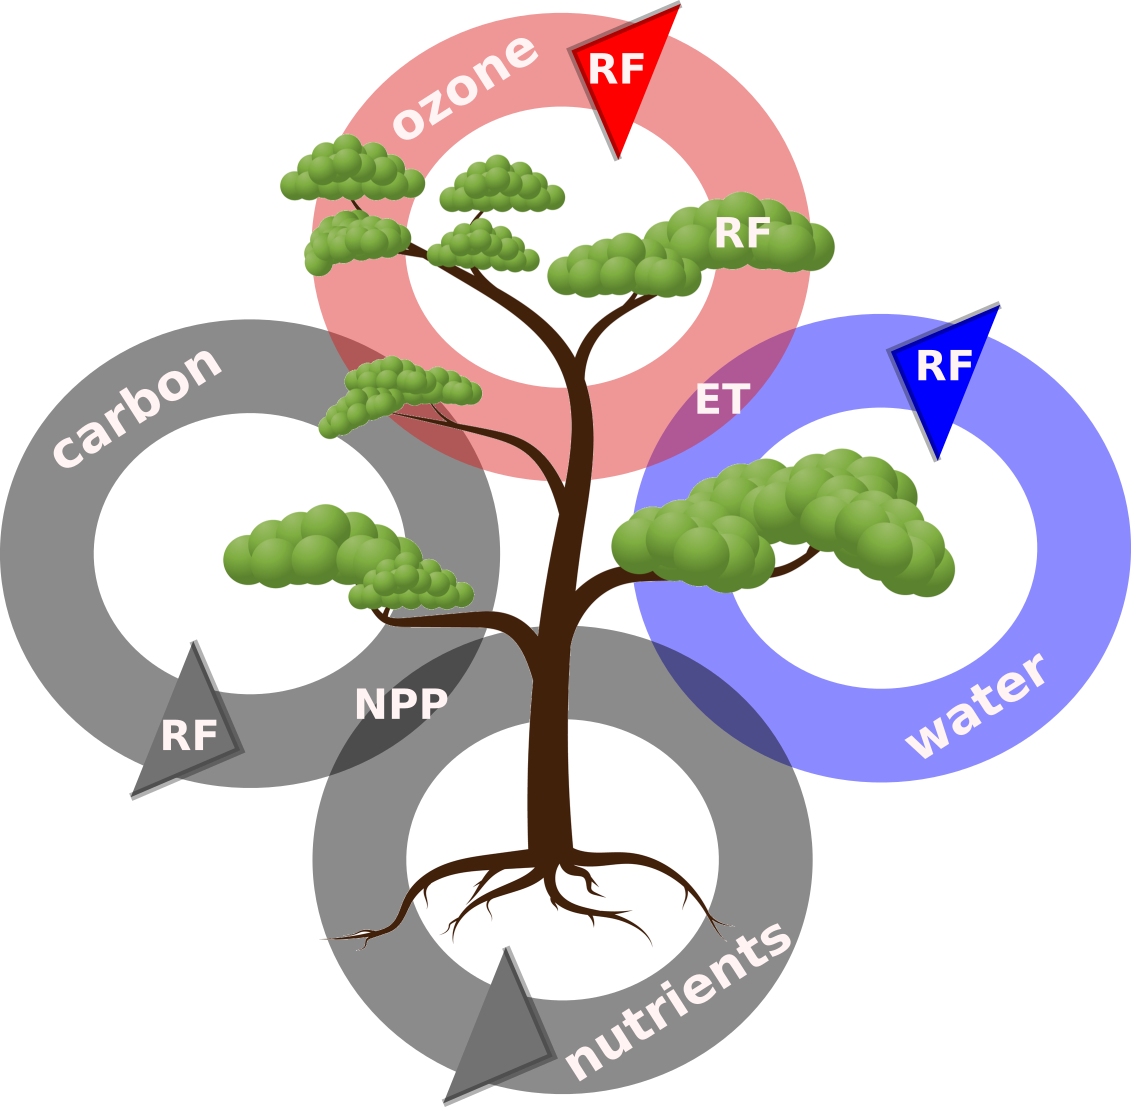
\includegraphics[width=0.48\textwidth]{ozone_es_scheme}
  \caption{Schematic view of the importance of ozone in \glspl{esm}. \textbf{\color{red}Ozone} inflicts damage to vegetation. Ozone affects photosynthesis negatively and hence \gls{npp} (\textbf{\color{darkgray}$\rightarrow$ carbon cycle}). Ozone affects opening and closing of stomata (positively and negatively) and hence \gls{et} of plants (\textbf{\color{blue}$\rightarrow$ water cycle}). Both affect the processing of nutrients (\textbf{\color{darkgray}$\rightarrow$ nutrient cycle}). Ozone damage on vegetation causes positive and negative feedback on tropospheric ozone concentrations and hence on air quality and \gls{rf} \parencite{Nat:Sitch2007}.}
  \label{fig:ozone_esm_scheme}
  \glsreset{npp}
  \glsreset{et}
  \glsreset{rf}
\end{figure}
%\end{wrapfigure}

Besides air quality considerations, \textbf{ozone interferes with the climate and Earth system both directly and indirectly}. Directly ozone affects the radiative forcing through its absorbance in both long and short wave bands and hence contributes to climate change. Indirectly ozone affects climate and air quality through ozone impacts on vegetation, which stand at the center of the proposed research. A high \gls{cuo} leads to considerably visible (e.g. necrosis, early senescence) and invisible damage (e.g. root growth) on vegetation \parencite{GCB:Mills2011}.

As illustrated in Fig.~\ref{fig:ozone_esm_scheme}, ozone effects on vegetation interfere with several sensitive components of the Earth system. \textbf{\color{red}Ozone damage} reduces plant photosynthesis and stomatal conductance. Ozone affects the \textbf{\color{darkgray}carbon cycle} through a reduced photosynthesis capacity and subsequent reduction in \gls{npp} and \gls{gpp}, which has consequences on the \textbf{\color{darkgray}nutrient cycle}. At the same time, physical damage will alter \gls{et} of the plant and hence the \textbf{\color{blue}water cycle}. All of these effects will affect the \gls{rf} and hence climate. Depending on the species and severity of damage both a reduction \parencite{Oe:Lombardozzi2012} or an increase (known as stomata sluggishness) \parencite{SR:Hoshika2015} have been reported. Accounting for ozone induced reduction of stomatal conductance and photosynthesis independently, \textcite{BGS:Lombardozzi2012} could improve model projections of changes in \gls{gpp} and transpiration on global scales.

In \textbf{our current understanding of photosynthesis at the plant physiological level}, maximum electron transport rate ($\mathrm{J_{max}}$) and maximum carboxylation efficiency ($\mathrm{V_{cmax}}$) are key parameters. Empirically it was found that ozone damage leads to a reduction of both $\mathrm{J_{max}}$ and $\mathrm{V_{cmax}}$ \parencite{EJA:Emberson2018}. Because the ratio $\mathrm{J_{max}}$:$\mathrm{V_{cmax}}$ is found to be constant (even under ozone exposure), first order effects of ozone induced damage can be modeled by a relative reduction in $\mathrm{J_{max}}$ or $\mathrm{V_{cmax}}$ alone. A simple linear relationship relates the relative reduction of $\mathrm{J_{max}}$ or $\mathrm{V_{cmax}}$ with the \gls{cuo} \parencites{BGS:Franz2017}{BGS:Franz2018}. \textcite{BGSD:Franz2020} showed that the impact of potential ozone damage on vegetation under climate change scenarios with explicit modeling on the plant physiological level has the potential to suppress projected gains in \gls{gpp} by increased nitrogen fertilization. These results, however, are associated with some uncertainty as they are based on a model without online atmospheric chemistry. The offline coupling of a land model to ozone concentrations provided from another \gls{ccm} leads to inconsistencies due to differences in land use and surface roughness and hence dry deposition velocities between the models. Given that the provided ozone concentrations from the \gls{ccm} are already in equilibrium with its own dry deposition scheme, a projected reduced uptake due to ozone damage would change the equilibrium concentration if coupled. \textbf{To study the effects of ozone on vegetation and the feedback on air quality in a fully consistent manner, a two-way coupling between the land and atmosphere components is essential.}\\

Here, we aim to integrate state-of-the-art process understanding at the vegetation level into a \gls{esm} with coupled atmospheric chemistry and state-of-the-art nutrient limited carbon sequestration to study the effects of ozone damage and thermal stress on vegetation and the resulting feedback on air quality and climate.

\section{Own contributions}
\label{sec:contrib}
The importance of ozone in the Earth system extends from large scales (stratospheric chemistry, dynamics, and radiation balance) to the smallest scales (damage on cellular level in plants). Following its trail, the applicant first studied \textbf{ozone depletion and future trends in the stratosphere} using the \gls{ccm} \gls{emac} model. In this respect the research activities primarily focused on future trends of biogenic brominated \gls{vsls} emitted from the ocean and the combined influence of sulfur aerosols \parencite{ACP:Falk2017}. In this study an increase of future ocean-atmosphere flux of brominated \gls{vsls} of $8-10\,\%$ compared to present day was found. A subsequent decrease in the tropospheric mixing ratios of brominated \gls{vsls} and an increase in the lower stratosphere are attributed to changes in atmospheric chemistry and transport and a reduced bromine impact on stratospheric ozone at the end of the 21st century was found compared to the present day.

The episodic \textbf{\glspl{ode} from the polar spring-time boundary layer} which are associated with suddenly occurring high bromide abundances (bromine explosions) lead the applicants way to model development, precisely the implementation of a bromine release mechanism based on \textcite{ACP:Toyota2011} in the \gls{emac} model. Many aspects of the observed bromine enhancement and associated \glspl{ode} in both polar regions could be reproduced by the model including the applicants extension which paved the way for testing of bromine release mechanisms in a global model \parencite{GMD:Falk2018}.

Subsequently the applicant’s research focused on ozone at lower levels. As a major sink of ozone in the troposphere is dry deposition, the applicant turned her eye towards this problem and integrated the \textbf{variable uptake of ozone by the land biosphere} into the scheme of the Oslo \gls{ctm}~3 \parencite{GMD:Falk2019}. This work has substantially improved ozone dry deposition velocities and abundance to vegetated surfaces in the model, and drew attention to the need for more mechanistic descriptions of dry deposition to non vegetated surfaces.

In the following, the applicants work focused in detail on the representation of \textbf{ozone damage with a special focus on subarctic biomes} \parencites{ICPTF:Falk2021}{EGU:Falk2021}. The analysis of the \gls{do3se} model results revealed that standard parameters optimized for central Europe may lead to significant underestimation of damage inflicted to vegetation acclimated to subarctic climates. The risk posed on subarctic biomes by the progressing climate change and a prolongation of the growing season may therefore be underestimated.

Last but not least, the applicant studied at the smallest scales the \textbf{process-based impact of ozone on the leaf-level} and implemented the \textbf{representation of ozone damage on nitrogen utilization in \gls{clm}~5.0}. First results were presented at the \gls{cesm} Land Model \& Biogeochemistry Working Group meeting \parencite{CESMWP:Falk2021}. This work is the foundation for the proposed development and analytical work in this project. This work indicated that the impact of ozone damage on \gls{gpp} strongly depends on the occurrence of the damage relative to the seasonal cycle of the vegetation.

Publications of these last two works are currently in preparation.
